% arara: lualatex: { shell: yes, interaction: nonstopmode, synctex: yes}
% arara: lualatex: { shell: yes, interaction: nonstopmode, synctex: yes}
% sarara: lualatex: { shell: yes, action: nonstopmode, synctex: yes}
% ssarara: lualatex: { shell: yes, action: nonstopmode, synctex: yes}
% asarara: lualatex: { shell: yes, action: nonstopmode, synctex: yes,  options: "-output-directory=_build"}
% asarara: lualatex: { shell: yes, action: nonstopmode, synctex: yes,  options: "-output-directory=_build"}
\documentclass{article}
\usepackage[ngerman]{babel}
\usepackage[no-math]{fontspec}

% \directlua{os.execute("cp basic/UbuntuL.ttf UbuntuL.ttf")}
% \directlua{os.execute("cp basic/UbuntuL.ttf UbuntuL.ttf")}
% \directlua{os.execute("c  p basic/UbuntuL.ttf UbuntuL.ttf")}

\usepackage{mwe}
\usepackage{luacode}
\usepackage{shellesc}
% \documentclassw[11pt, a4paper,ngerman]{article}
\usepackage{../../latexBasic/basicff}


\usetikzlibrary{patterns} % preamble
\tcbuselibrary{skins} % preamble

\usepackage{tikz}
% \usepackage{PTSansNarrow}
\usetikzlibrary{matrix}

\usepackage{pgfplots}
\pgfplotsset{
 compat=newest
  }
\tcbset{colframe=red!75!black}
\newenvironment{proggen}{\begin{center}}{\end{center}}

\usepackage{array}
% \setmainfont[Path=/Applications/Microsoft Word.app/Contents/Resources/Fonts/]{Calibri.ttf}
% \setsansfont[Path=/Applications/Microsoft Word.app/Contents/Resources/Fonts/]{Calibri.ttf}
% \setmonofont[Path=/Applications/Microsoft Word.app/Contents/Resources/Fonts/]{Calibri.ttf}


\setmainfont[Numbers=OldStyle, Path=../latexBasic/]{UbuntuL.ttf}
\setsansfont[BoldFont = Ubuntu-B ,Numbers=OldStyle, Path=../latexBasic/]{UbuntuR.ttf}
\setmonofont[Numbers=OldStyle, Path=../latexBasic/]{UbuntuMonoR.ttf}
% \liningnums{\textbf{}}
% \oldstylenums{\textbf{}}


\newcolumntype{C}[1]{>{\centering\arraybackslash}m{#1}}

\oddsidemargin-10mm
\title{
\color{white}
 $\bullet$ \\ $\bullet$ \\ $\bullet$ \\
 \color{black}
 % \color{white}
 % $\bullet$ \\
 \color{black}
 \begin{center}
   GCODEview \\
   \color{white}
   $\bullet$ \\
   \color{black}
   Formula Mundi
 \end{center}
\color{white}
$\bullet$ \\
\color{black}
 \begin{center}
 % \includegraphics[scale=0.5]{./pictures/CaptainWarschburger.jpg}
\end{center}
 % \includegraphics{./pictures/wohnzimmer.png}
}
% \includegraphics{./pictures/asrock.png} Q1900M \\ \color{white} $\bullet$ \\ $\bullet$ \\ $\bullet$ \\ \color{black} \\ \apple \\ 10.10.3

\author{Daniel Krah}
% \date{1.6.2015}

\begin{document}
% \AddToShipoutPicture{\BackgroundPic}
\maketitle%
\newpage%
 % \tableofcontents%
% \newpage
%==================================================================================

% \newpage
% \sect{Überblick}
% \section{Überblick}


\section{Vorwort}

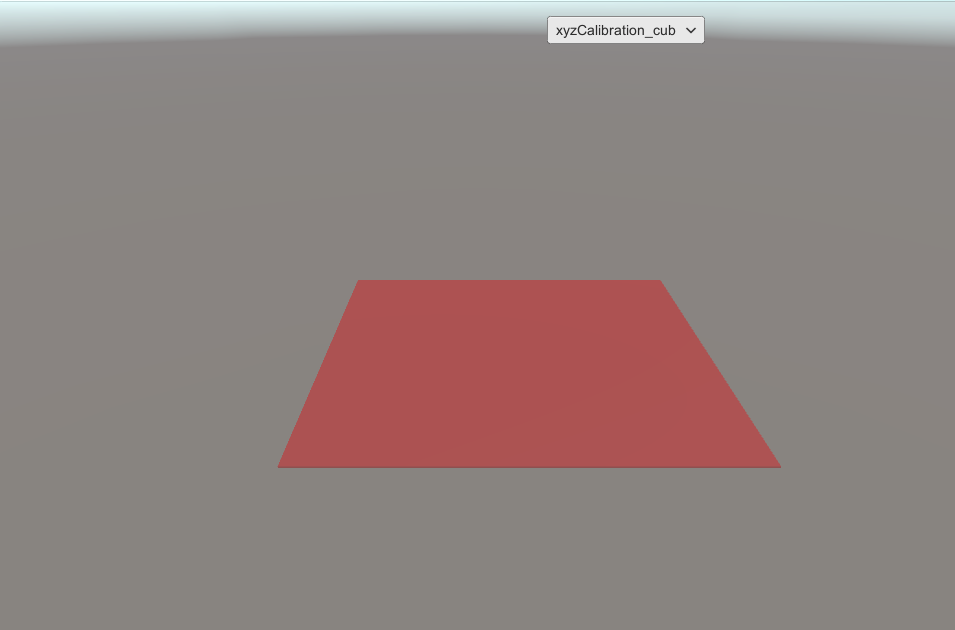
\includegraphics[width=\paperwidth-3cm]{./pictures/dropdown.png}


\section{.gcode Parser}

\subsection{Basiswerte}

\monocodebox{sh}{Slicersetting Ideamaker:}{./codesnippets/xyzCalibration_cube.gcode
}{false}{0}{12}

Zur Anzeige benötigte Werte:
\begin{itemize}
  \item Dimension (Breite, Tiefe, Höhe, Düsendurchmesser)
  \item Filament Diameter
  \item Plate Shape (Rechteckig / Rund)
\end{itemize}

\subsection{Startcode}
\monocodebox{sh}{Druck Startcode}{./codesnippets/xyzCalibration_cube.gcode
}{false}{13}{27}

Hier werden vereinfacht nur die Temperaturen gesetzt und mit \textbf{G28}die Home Position angefahren.

\newpage

\subsection{Startcode Nozzle prime}
\monocodebox{sh}{Druck Startcode Nozzle prime}{./codesnippets/xyzCalibration_cube.gcode
}{false}{26}{35}

Hier wird außerhalb des Druckbereiches Material in die Düse gedrückt.
Dies ist nötig damit dann beim drucken des Models schon Material am Ausgang der Düse ist.

\subsection{Extruder-Mode}
\monocodebox{sh}{Extruder-Mode}{./codesnippets/xyzCalibration_cube.gcode
}{false}{36}{36}

Diese Zeile ist wichtig da sie festlegt wie die nachfolgenden G codes interpretiert werden sollen.\\

Es gibt verschiedene Arten der Befehle:\\

N: Line number\\
G0 : Rapid Move\\
G1 : Linear Move\\
% \monocodebox{sh}{Speedtest mittels Terminal:}{./codesnippets/speedtest.sh}{false}{0}{9999999}

% \includegraphics[scale=0.5]{./pictures/streamingarten.png}




%
% \begin{tabular}{ll}
% \centering
% \glqq Text\grqq{} und \flqq Text\frqq  & \verb+ \glqq Text\grqq{} und \flqq Text\frqq+\\
% \glq Text\grq{} und \flq Text\frq  & \verb+ \glq Text\grq{} und \flq Text\frq+
% \end{tabular}





% \definecolor{fulda_green}{rgb}{.38,.74,.10}
% \definecolor{fulda_lightgreen}{rgb}{.64,.85,.40}
% \definecolor{fulda_lightgray}{gray}{.4}
% \definecolor{fulda_subtitle}{rgb}{.38,.74,.10}
% \definecolor{fulda_title}{gray}{.0}
% \definecolor{fulda_chapter}{rgb}{.38,.74,.10}
% \definecolor{fulda_section}{rgb}{.38,.74,.10}
% \definecolor{fulda_subsection}{gray}{.4}
% \definecolor{fulda_part}{gray}{1}
% \definecolor{fulda_partnumber}{rgb}{.79,1,.55}
% \definecolor{fulda_partback}{rgb}{.64,.85,.40}
% \definecolor{fulda_highlighttitle}{rgb}{.38,.74,.10}
% \definecolor{fulda_highlightbody}{rgb}{.79,1,.55}
% \definecolor{fulda_highlighttitletext}{gray}{1}
% \definecolor{lightgray}{rgb}{0.93,0.95,1.0}
% \definecolor{darkgreen}{RGB}{82,130,179}

% \input{strukturen.tex}
% \input{threadsProzesse.tex}

%=========================================================================================================================
%
%-------------END
\end{document}
